
%%% ADO.NET vs ORM like entity framework
%%% EF, Code first, TDD, DB-first?
%%%%% Lazy-eager loading?
%%%%% Query generation
%%%%% Pitfalls
% Reasoning over these
% Choice - and reason for choice
% Design of the database, and implementation details and reasoning
% Normalization too
% Relational model
\chapter{Arkitektur}\label{ch:arkitektur}

Dette afsnit omhandler hvilke arkitektur overvejelser der har været i projektet. Da et af målene med projektet er at lave en web-server som kan håndtere samtidighed mellem flere brugere, vil der være bestemte arkitekturer og overvejelser, som kan benyttes til at opnå målet. Herunder Distribuerede Systemer, RESTful Web API, Desktop Programming, Database design og Web design.

Fremgangsmåden i projektet har været bottom-up, forstået på den måde, at rækkefølgen af hver feature er håndteret i rækkefølgen:
\begin{itemize}\label{procedure}
    \item Database-struktur design (relationel model)
    \item Oprettelse af database tabel(ler)
    \item Design af model (C\#)
    \item Oprettelse af model (C\#)
    \item Oprettelse af DAO
    \item Oprettelse af Controller
    \item Gennemførsel af tests
    \item Simpelt design af front-end
    \item Pænt design af front-end
\end{itemize}

\section{Distribueret System}\label{sec:distSys}
% I need some help explaining better what OSI, TCP/IP, and how all these layers and services relate to that
Dette projekt havde et krav om at være et distribueret system, bestående af flere services, som skulle kunne kommunikere med hinanden gennem en API. API'en er en kontrakt, som sørger for at flere systemer kan kommunikere med hinanden\cite{API}. Dette foregår gennem HTTP protokoller\cite{http}.
Som navnet "distribueret system" hentyder til, så skal disse services ikke være afhængige af hinanden - de skal decouples\cite{decoupling} og destribueres. Der er flere muligheder når det kommer til design af sådan et system. Det kan designes ud fra en lagdelt arkitektur som OSI eller TCP/IP\cite{osi_tcp}, og gøre brug af MVC design-mønstret. I TCP/IP forekommer disse lag: Applikationslag, Transportlag, Netværkslag og Netværks interface.
Hvert lag tjener sit eget formål ift. resten af programmet.
For at gennemføre dette er der blevet brugt en 3-lags arkitektur, som indeholder et præsentationslag, logik lag, og data lag.

\begin{figure}
    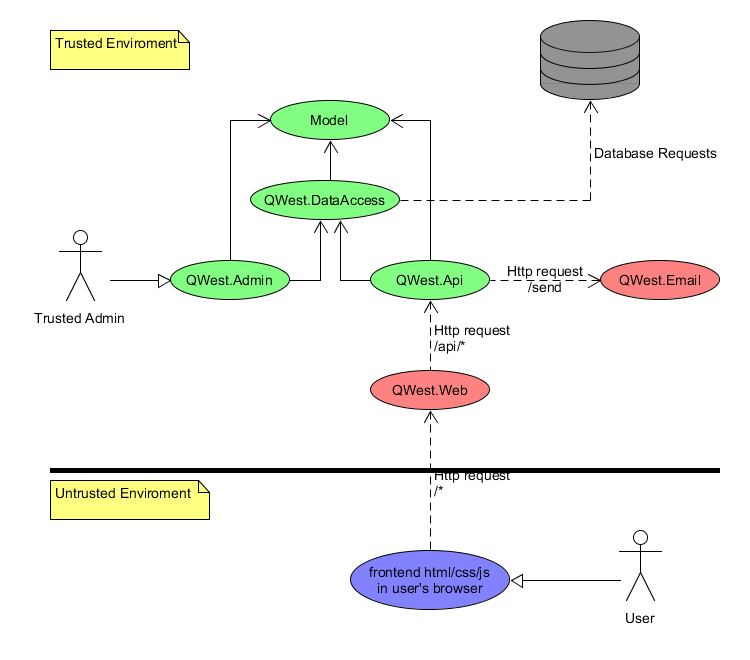
\includegraphics[width=\linewidth]{architecture.png}
    \caption{QWest arkitektur model.}
    \label{fig:architecture_model}
\end{figure}

I arkitektur modellen~\ref{fig:architecture_model} beskriver ellipserne klienter, servicer, library projecter eller lignende, blå værende frontend html/css/js, rød værende node.js\cite{nodejs} og grøn værende C\#.
De stiplede linjer beskriver interprocess kommunikation, i dette diagram er det altid http forespørgsler eller forespørgsler til databasen.
De fuldt optrukkede linjer mellem intraprocess kommunikation, er oftest når et runtime af en art henter kode ind fra en anden del af projektet, fx QWest.Api dll'en som henter ind fra QWest.DataAccess dll'en.
Ud over dette, er modellen delt op i 2 dele, "trusted enviroment" og "untrusted enviroment". I "trusted enviroment" kan vi stole på at de forespørgsler vi modtager kommer fra os, så vi ikke behøver at tænke på ting som sikkerhed af autentificering. "untrusted enviroment" er hvor bruger input kommer fra, det kan være alt fra SQL injection angreb til helt et normalt bruger input.

\begin{figure}
    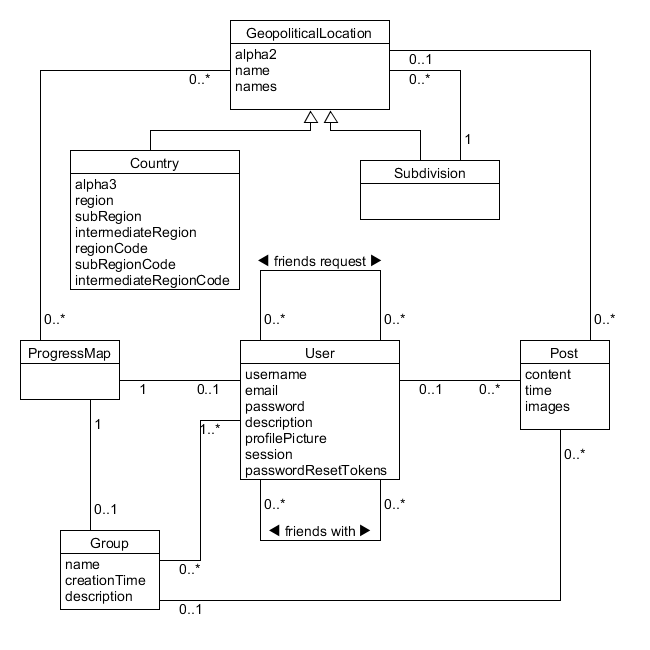
\includegraphics[width=\linewidth]{domain_model.png}
    \caption{QWest domænemodel.}
    \label{fig:domain_model}
\end{figure}

\subsection{Services}\label{sec:servicesArc}
Som nævnt tidligere, bruger man services til at håndtere kommunikation mellem de forskellige dele af programmet. Formålet er at gøre de forskellige dele uafhængige af hinanden så databasen ikke frit kan tilgås, så man kan skjule og ændre back-end uden at påvirke front-end og centralisere logikken i systemet. Disse er struktureret ud fra en 3-tier arkitektur\cite{3tier}, med Client, Logic og Data tiers.

I QWest er der følgende services:
\begin{itemize}\label{services}
    \item QWest.Api
    \item QWest.Email
    \item QWest.Web
\end{itemize}

Og De følgende klienter
\begin{itemize}\label{services}
    \item QWest.Admin
    \item QWest.Web frontend
\end{itemize}

QWest.Admin og QWest.Web frontend er henholdsvis administrator adgang og bruger adgang og indgår i Client-tier. QWest.Admin åbner Desktop applikationen, hvor hvert land kan opdateres manuelt. Det skulle så være muligt hvert år at opdatere informationerne på hvert land én gang om året. QWest.Admin benytter sig ikke af Web og Email servicen, da det i dette projekt er vurderet, at det ikke er nødvendigt med front-end til administration. 

\begin{figure}
    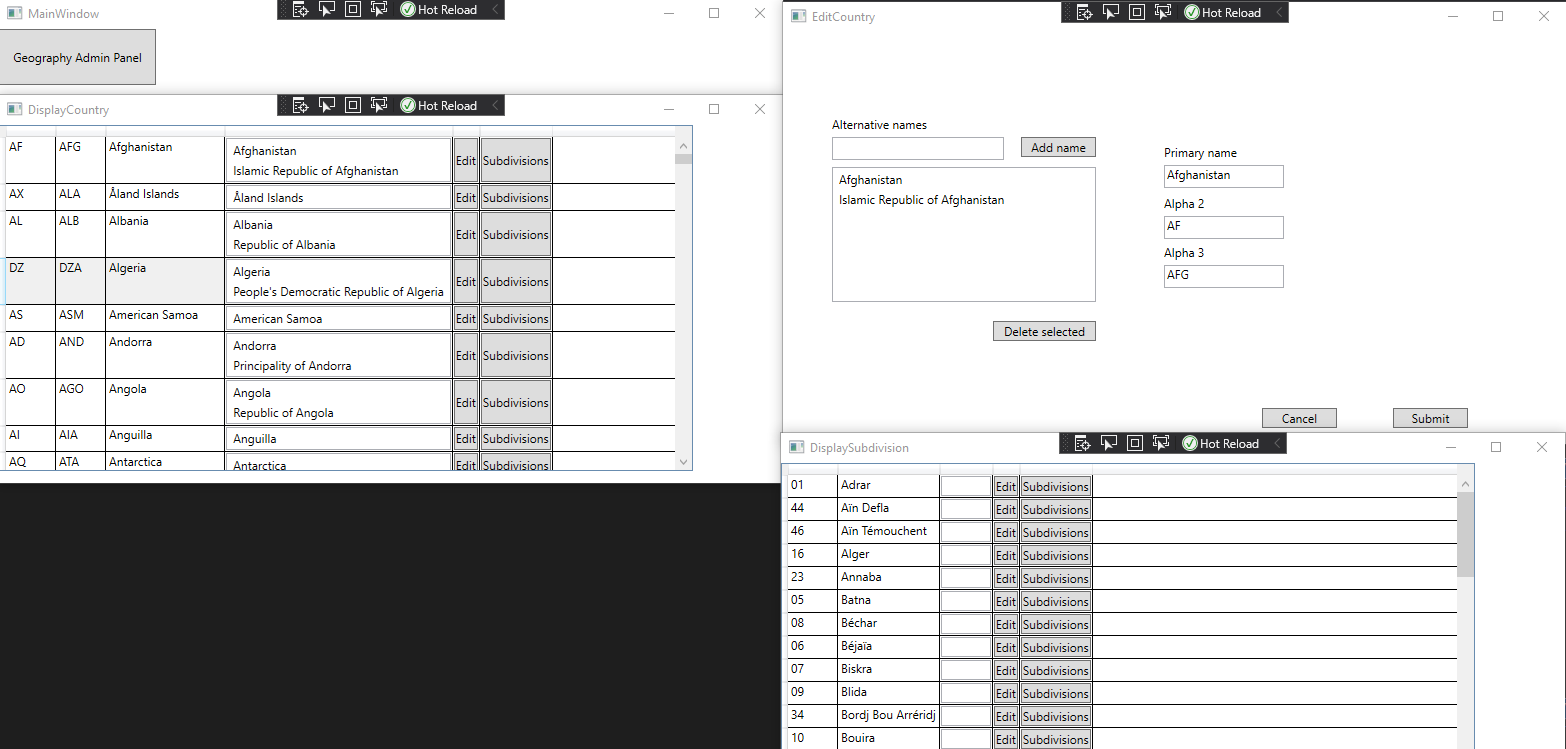
\includegraphics[width=\linewidth]{admin_panel.png}
    \caption{QWest.Admin vinduet, med undervinduer.}
    \label{fig:admin_panel}
\end{figure}

QWest.Web er en frontend og brugerens klient, og hører derfor også under Client-tier. Der bliver genereret HTML i QWest.Web, som kan vises i en browser. QWest.Web frontend kommunikerer med vores REST service QWest.Api gennem QWest.Web, der fungerer som en proxy, og sender http forespørgsler. Forespørgsler sendes med teksten \texttt{/api/} til QWest.Api, hvor metoder i backend så kan tilgås. QWest.Email er en service dedikeret til at sende emails til brugere og bruges kun til at sende mail til nulstilling af password. QWest.Email er en meget lille service, omrking 50 linjer kode, og der kunne nemt argumenteres for, at det skulle være en del af QWest.Api. Dette var originalt planen, men der eksisterer ikke nogle "out-of-the-box" biblioteker, som ikke kræver at en SMTP server for C\#, men kun node.js, og dette reducerer mulighederne for at sætte en SMTP server op eller bare lave email til et seperat service skrevet i node.js.


\section{RESTful Web API}\label{sec:REST}
Vores REST API, QWest.Api, er en service for sig selv, hvis primære job er at håndtere logikken for brugerens interaktion med platformens persistente data. Dette er derfor under Logic-tier. QWest.Api sørger blandt andet for, at vi er sikre på, at data der håndteres giver mening i forhold til domænet (fx at vi ikke opretter en gruppe, uden personer i gruppen) og checker om brugeren er autentificeret.

QWest.Api bruger frameworket ASP.NET framework Web Api, sammen med OWIN\cite{Owin} til middleware og Json.NET til serializering og deserializering a JSON data.

QWest.Api bruger JSON som representation metoden, dette gøres eftersom at JSON er en af de mest populære måder af serializere data, ud over det er JSON både læseligt for mennesker sammentidig med at bruge mindre plads end andre menneskelæselig alternativer som XML. JSON er også bygget ind i javascript, hvilket gør det et næmt valg dag vores primære bruger af dette API kommer til at være QWest.Web frontend som er 100\% javascript at det skal køre i en browser
% Cite JSON^^

\section{Desktop Programming}\label{sec:deskProgramming}
% This is the QWest.Admin stuff

\section{Database}\label{sec:database}
Det sidste tier i 3-tier arkitekturen er selvfølgelig databasen. Databasen til projektet er oprettet med MSSQL\cite{MSSQL}. Til trods for at der findes andre SQL sprog end Microsoft's, blev MSSQL valgt fordi det er det vi i udviklingsteamet kender bedst til. Det ville være risikabelt at bruge en ubestemt mængde af tid på at sætte sig ind i et andet SQL system - især når vi i gruppen allerede har en god forståelse for MSSQL og skolen tildeler en gratis MSSQL server. Til gengæld er der taget højde for, at det skulle være muligt at implementere et andet SQL system - dette er gjort med DAO'er. DAO\cite{dao} designmønstret er gennemgående i projektet og forefindes i koden under QWest.DataAccess. Selve MSSQL implementationen findes i Mssql mappen. Der er valgt at bruge disse DAO og SQLConnections fremfor ORM %Yea but why?

\begin{figure}
    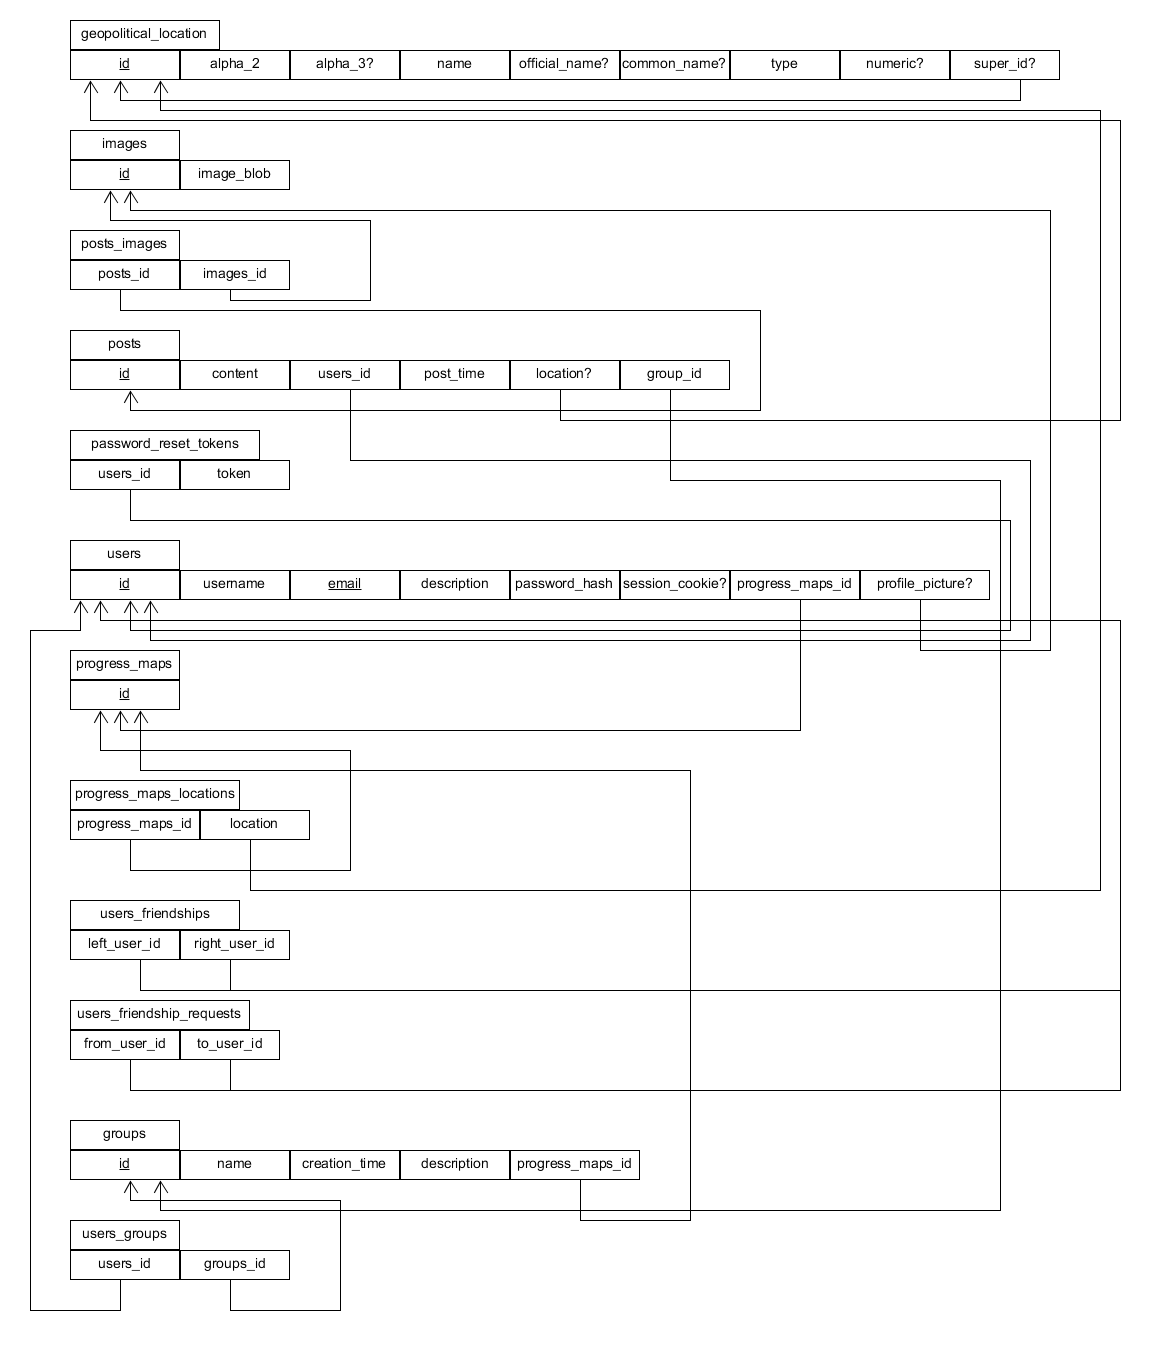
\includegraphics[width=\linewidth]{relational_model.png}
    \caption{QWest relationel model for databasen.}
    \label{fig:relational_model}
\end{figure}

\texttt{users} er omdrejningspunktet i databasen, da \texttt{users} er forbundet med \texttt{progress\_maps}, \texttt{posts}, \texttt{password\_reset\_tokens}, \texttt{users\_friendships}, \texttt{users\_friendship\_requests} og \texttt{users\_groups}. Disse forbinder så til resten af tabellerne, hvor \texttt{posts} har \texttt{posts\_images}, som har \texttt{images}. \texttt{progress\_maps} er forbundet med \texttt{geopolitical\_location}, gennem \texttt{progress\_maps\_locations}. \texttt{groups} er forbundet gennem \texttt{users\_groups}.

I domæne modellen, figur \ref{fig:domain_model}, ses forholdene mellem klasserne, som er belæg for de forskellige sammenkoblinger af tabellerne så modellerne afspejler hinanden. Databasen opfylder ikke samtlige krav til BCNF\cite{bcnf}. \texttt{name} på \texttt{geopolitical\_locations} og manglen på en seperat \texttt{subregions} tabel til \texttt{geopolitical\_location}. \texttt{name} er ikke atomisk, og kan indeholde flere navne på det samme land. Dette skyldes at lande som regel har flere officielle navne. Eksempelvis kan Storbrittanien hedde "United Kingdom", "Storbrittanien" og "UK", men stadig være det samme på alle andre områder. Såfremt et land har flere officielle navne, så lagres de i ét felt da det beskriver den samme tuple.

\section{Web design}\label{sec:webdesign}
Web-klienten til brugeren kan tilgås igennem en browser. %uhhhhhh idk what more write
\subsection{Back-end and logic}\label{sec:backend}
Logikken er skrevet i Javascript og JQuery, som håndtere alle funktioner på hjemmesiden. Der bruges bl.a. Javascript og JQuery til dynamisk at indsætte diverse knapper, venner, grupper, og opslag, ud fra informationerne lagret i databasen. Det er altså Javascript og JQuery som sørger for, at information fra front-end kan blive sendt til back-end og databasen, ved at kalde QWest.Api som indeholder de forskellige Controller-klasser. %More in implementation
\subsection{Front-end and usability}\label{sec:frontend}
Selve front-end er designet ud fra enkelte principper: Top og bund af hver subdomæne skal være nogenlunde ens, knapper skal være store og tydelige, og siderne skal kunne vises på forskellige skærmstørrelser og devices. Al styling er foregået med CSS. Hvordan alt dette er implementeret vil gennemgås i implementation afsnittet. %needs more here? Otherwise we can write about it in implementation
